\documentclass[twoside]{book}

% Packages required by doxygen
\usepackage{calc}
\usepackage{doxygen}
\usepackage{graphicx}
\usepackage[utf8]{inputenc}
\usepackage{makeidx}
\usepackage{multicol}
\usepackage{multirow}
\usepackage{textcomp}
\usepackage[table]{xcolor}

% Font selection
\usepackage[T1]{fontenc}
\usepackage{mathptmx}
\usepackage[scaled=.90]{helvet}
\usepackage{courier}
\usepackage{amssymb}
\usepackage{sectsty}
\renewcommand{\familydefault}{\sfdefault}
\allsectionsfont{%
  \fontseries{bc}\selectfont%
  \color{darkgray}%
}
\renewcommand{\DoxyLabelFont}{%
  \fontseries{bc}\selectfont%
  \color{darkgray}%
}

% Page & text layout
\usepackage{geometry}
\geometry{%
  a4paper,%
  top=2.5cm,%
  bottom=2.5cm,%
  left=2.5cm,%
  right=2.5cm%
}
\tolerance=750
\hfuzz=15pt
\hbadness=750
\setlength{\emergencystretch}{15pt}
\setlength{\parindent}{0cm}
\setlength{\parskip}{0.2cm}
\makeatletter
\renewcommand{\paragraph}{%
  \@startsection{paragraph}{4}{0ex}{-1.0ex}{1.0ex}{%
    \normalfont\normalsize\bfseries\SS@parafont%
  }%
}
\renewcommand{\subparagraph}{%
  \@startsection{subparagraph}{5}{0ex}{-1.0ex}{1.0ex}{%
    \normalfont\normalsize\bfseries\SS@subparafont%
  }%
}
\makeatother

% Headers & footers
\usepackage{fancyhdr}
\pagestyle{fancyplain}
\fancyhead[LE]{\fancyplain{}{\bfseries\thepage}}
\fancyhead[CE]{\fancyplain{}{}}
\fancyhead[RE]{\fancyplain{}{\bfseries\leftmark}}
\fancyhead[LO]{\fancyplain{}{\bfseries\rightmark}}
\fancyhead[CO]{\fancyplain{}{}}
\fancyhead[RO]{\fancyplain{}{\bfseries\thepage}}
\fancyfoot[LE]{\fancyplain{}{}}
\fancyfoot[CE]{\fancyplain{}{}}
\fancyfoot[RE]{\fancyplain{}{\bfseries\scriptsize Generated on Tue Jan 21 2014 15\-:20\-:00 for Ui\-O F\-Y\-S4411 by Doxygen }}
\fancyfoot[LO]{\fancyplain{}{\bfseries\scriptsize Generated on Tue Jan 21 2014 15\-:20\-:00 for Ui\-O F\-Y\-S4411 by Doxygen }}
\fancyfoot[CO]{\fancyplain{}{}}
\fancyfoot[RO]{\fancyplain{}{}}
\renewcommand{\footrulewidth}{0.4pt}
\renewcommand{\chaptermark}[1]{%
  \markboth{#1}{}%
}
\renewcommand{\sectionmark}[1]{%
  \markright{\thesection\ #1}%
}

% Indices & bibliography
\usepackage{natbib}
\usepackage[titles]{tocloft}
\setcounter{tocdepth}{3}
\setcounter{secnumdepth}{5}
\makeindex

% Hyperlinks (required, but should be loaded last)
\usepackage{ifpdf}
\ifpdf
  \usepackage[pdftex,pagebackref=true]{hyperref}
\else
  \usepackage[ps2pdf,pagebackref=true]{hyperref}
\fi
\hypersetup{%
  colorlinks=true,%
  linkcolor=blue,%
  citecolor=blue,%
  unicode%
}

% Custom commands
\newcommand{\clearemptydoublepage}{%
  \newpage{\pagestyle{empty}\cleardoublepage}%
}


%===== C O N T E N T S =====

\begin{document}

% Titlepage & ToC
\hypersetup{pageanchor=false}
\pagenumbering{roman}
\begin{titlepage}
\vspace*{7cm}
\begin{center}%
{\Large Ui\-O F\-Y\-S4411 }\\
\vspace*{1cm}
{\large Generated by Doxygen 1.8.6}\\
\vspace*{0.5cm}
{\small Tue Jan 21 2014 15:20:00}\\
\end{center}
\end{titlepage}
\clearemptydoublepage
\tableofcontents
\clearemptydoublepage
\pagenumbering{arabic}
\hypersetup{pageanchor=true}

%--- Begin generated contents ---
\chapter{Hierarchical Index}
\section{Class Hierarchy}
This inheritance list is sorted roughly, but not completely, alphabetically\-:\begin{DoxyCompactList}
\item exception\begin{DoxyCompactList}
\item \contentsline{section}{Exception}{\pageref{class_exception}}{}
\end{DoxyCompactList}
\item \contentsline{section}{Hydrogen\-Lin\-Alg\-Solver}{\pageref{class_hydrogen_lin_alg_solver}}{}
\end{DoxyCompactList}

\chapter{Class Index}
\section{Class List}
Here are the classes, structs, unions and interfaces with brief descriptions\-:\begin{DoxyCompactList}
\item\contentsline{section}{\hyperlink{class_exception}{Exception} }{\pageref{class_exception}}{}
\item\contentsline{section}{\hyperlink{class_hydrogen_lin_alg_solver}{Hydrogen\-Lin\-Alg\-Solver} }{\pageref{class_hydrogen_lin_alg_solver}}{}
\end{DoxyCompactList}

\chapter{Class Documentation}
\hypertarget{class_exception}{\section{Exception Class Reference}
\label{class_exception}\index{Exception@{Exception}}
}


{\ttfamily \#include $<$types.\-h$>$}

Inheritance diagram for Exception\-:\begin{figure}[H]
\begin{center}
\leavevmode
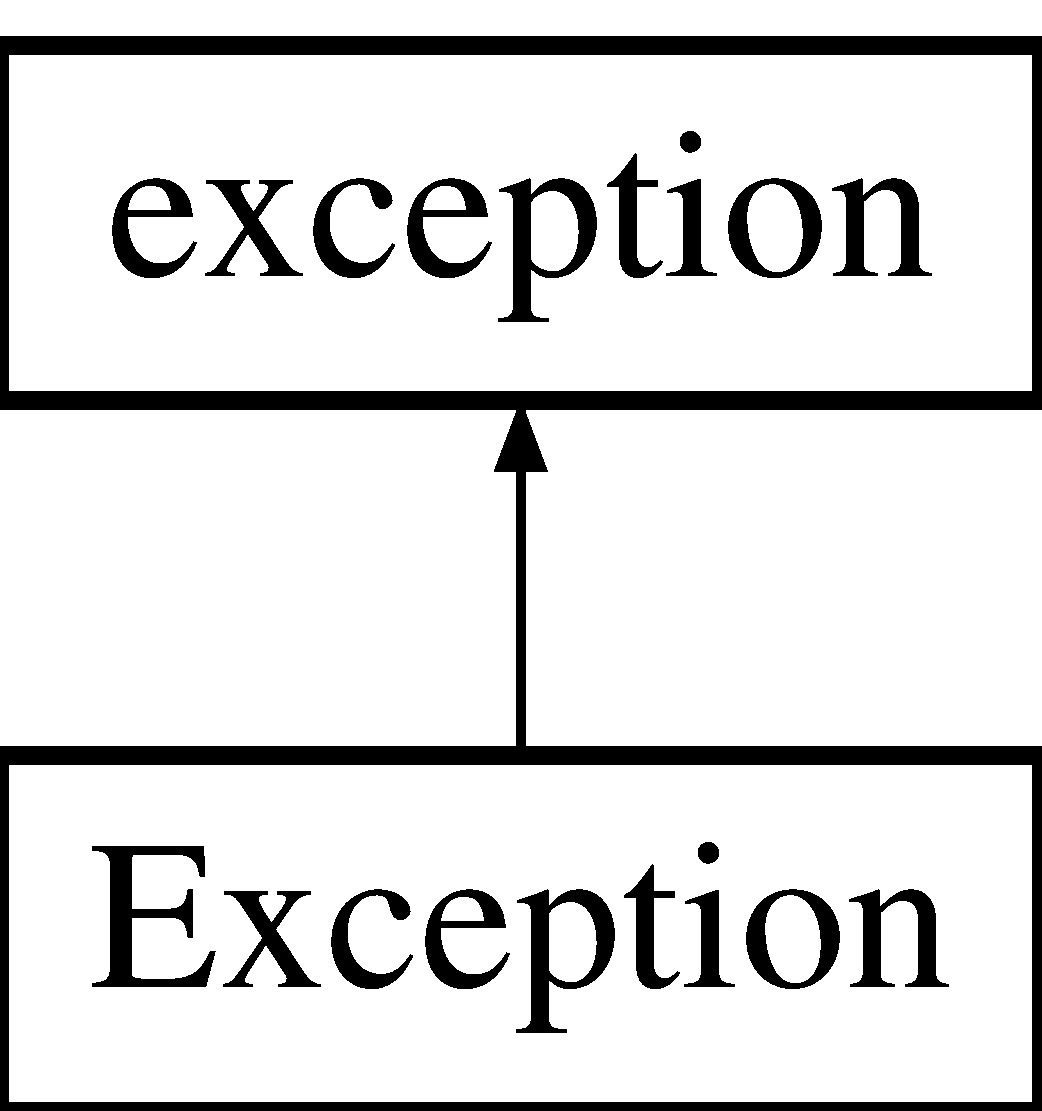
\includegraphics[height=2.000000cm]{class_exception}
\end{center}
\end{figure}
\subsection*{Public Member Functions}
\begin{DoxyCompactItemize}
\item 
\hypertarget{class_exception_a4821522f27880a019004c8324af2b8bd}{{\bfseries Exception} (str msg)}\label{class_exception_a4821522f27880a019004c8324af2b8bd}

\item 
\hypertarget{class_exception_a45642915395d3b813fedc2593fbcb8bb}{const char $\ast$ {\bfseries what} () const   throw ()}\label{class_exception_a45642915395d3b813fedc2593fbcb8bb}

\end{DoxyCompactItemize}


\subsection{Detailed Description}
exception wrapper to provide \hyperlink{class_exception}{Exception(string)} \begin{DoxyAuthor}{Author}
Felix Hekhorn \href{mailto:felix.hekhorn@student.uni-tuebingen.de}{\tt felix.\-hekhorn@student.\-uni-\/tuebingen.\-de} 
\end{DoxyAuthor}


The documentation for this class was generated from the following file\-:\begin{DoxyCompactItemize}
\item 
cpp/types.\-h\end{DoxyCompactItemize}

\hypertarget{class_hydrogen_lin_alg_solver}{\section{Hydrogen\-Lin\-Alg\-Solver Class Reference}
\label{class_hydrogen_lin_alg_solver}\index{Hydrogen\-Lin\-Alg\-Solver@{Hydrogen\-Lin\-Alg\-Solver}}
}


{\ttfamily \#include $<$hydrogenlinalgsolver.\-h$>$}

\subsection*{Public Member Functions}
\begin{DoxyCompactItemize}
\item 
\hyperlink{class_hydrogen_lin_alg_solver_a2532bd8f2a6c38f8019be1499d7d8ad5}{Hydrogen\-Lin\-Alg\-Solver} (uint N\-\_\-step, dbl R\-\_\-max, dbl Z=1., uint l=0)
\begin{DoxyCompactList}\small\item\em constructor \end{DoxyCompactList}\item 
\hypertarget{class_hydrogen_lin_alg_solver_a11597d0b5728926bdb28ade85621bb94}{void \hyperlink{class_hydrogen_lin_alg_solver_a11597d0b5728926bdb28ade85621bb94}{run} ()}\label{class_hydrogen_lin_alg_solver_a11597d0b5728926bdb28ade85621bb94}

\begin{DoxyCompactList}\small\item\em solves the problem \end{DoxyCompactList}\item 
void \hyperlink{class_hydrogen_lin_alg_solver_a6bc283dc14305bc00b4d38860a891448}{log\-V} (str path)
\begin{DoxyCompactList}\small\item\em log\-V loggs the potential to a file \end{DoxyCompactList}\end{DoxyCompactItemize}


\subsection{Detailed Description}
Defines the main class for solving standard hydrogen waveequation via eigenwertsolver

Solves the standard hydrogen waveequation by using the eigenwertequation uses at all times natural units

\begin{DoxyAuthor}{Author}
Felix Hekhorn \href{mailto:felix.hekhorn@student.uni-tuebingen.de}{\tt felix.\-hekhorn@student.\-uni-\/tuebingen.\-de} 
\end{DoxyAuthor}


\subsection{Constructor \& Destructor Documentation}
\hypertarget{class_hydrogen_lin_alg_solver_a2532bd8f2a6c38f8019be1499d7d8ad5}{\index{Hydrogen\-Lin\-Alg\-Solver@{Hydrogen\-Lin\-Alg\-Solver}!Hydrogen\-Lin\-Alg\-Solver@{Hydrogen\-Lin\-Alg\-Solver}}
\index{Hydrogen\-Lin\-Alg\-Solver@{Hydrogen\-Lin\-Alg\-Solver}!HydrogenLinAlgSolver@{Hydrogen\-Lin\-Alg\-Solver}}
\subsubsection[{Hydrogen\-Lin\-Alg\-Solver}]{\setlength{\rightskip}{0pt plus 5cm}Hydrogen\-Lin\-Alg\-Solver\-::\-Hydrogen\-Lin\-Alg\-Solver (
\begin{DoxyParamCaption}
\item[{uint}]{N\-\_\-step, }
\item[{dbl}]{R\-\_\-max, }
\item[{dbl}]{Z = {\ttfamily 1.}, }
\item[{uint}]{l = {\ttfamily 0}}
\end{DoxyParamCaption}
)}}\label{class_hydrogen_lin_alg_solver_a2532bd8f2a6c38f8019be1499d7d8ad5}


constructor 


\begin{DoxyParams}{Parameters}
{\em N\-\_\-step} & \\
\hline
{\em R\-\_\-max} & \\
\hline
{\em Z} & \\
\hline
{\em l} & \\
\hline
\end{DoxyParams}


\subsection{Member Function Documentation}
\hypertarget{class_hydrogen_lin_alg_solver_a6bc283dc14305bc00b4d38860a891448}{\index{Hydrogen\-Lin\-Alg\-Solver@{Hydrogen\-Lin\-Alg\-Solver}!log\-V@{log\-V}}
\index{log\-V@{log\-V}!HydrogenLinAlgSolver@{Hydrogen\-Lin\-Alg\-Solver}}
\subsubsection[{log\-V}]{\setlength{\rightskip}{0pt plus 5cm}void Hydrogen\-Lin\-Alg\-Solver\-::log\-V (
\begin{DoxyParamCaption}
\item[{str}]{path}
\end{DoxyParamCaption}
)}}\label{class_hydrogen_lin_alg_solver_a6bc283dc14305bc00b4d38860a891448}


log\-V loggs the potential to a file 


\begin{DoxyParams}{Parameters}
{\em path} & targetpath of file \\
\hline
\end{DoxyParams}


The documentation for this class was generated from the following files\-:\begin{DoxyCompactItemize}
\item 
cpp/hydrogenlinalgsolver.\-h\item 
cpp/hydrogenlinalgsolver.\-cpp\end{DoxyCompactItemize}

%--- End generated contents ---

% Index
\newpage
\phantomsection
\addcontentsline{toc}{chapter}{Index}
\printindex

\end{document}
